\chapter{简介}\label{chap:1}

当我们考虑学习的本质时, 通过与环境交互来学习这一想法可能是我们第一个想到的. 当幼儿玩耍、挥动手臂或者四下查看时, 他并没有一个实际的老师, 但他确实和环境有着直接的感觉、运动上的联系. 锻炼这一联系产生了丰富的关于因果的信息, 关于动作的结果的信息, 以及关于为了达到目标应该做什么的信息. 在我们的一生中, 这样的交互毫无疑问是关于我们所处的环境和关于我们自身的知识的主要来源. 无论是学习开车还是学习进行对话, 我们都敏锐地察觉到我们的环境会怎样地对我们的行为做出反应, 并且我们希望通过我们的行为影响结果. 从交互中学习是一个位于几乎所有的学习与智能理论之下的基本的想法.

在本书中我们探讨一种\emph{计算性}的从交互中学习的方法. 我们主要探讨理想化的学习情况, 并评估不同学习方法的效率\footnote{与心理学和神经科学的关系在\chapref{14}与\chapref{15}进行了概括.}, 而不是直接建立人与动物怎样学习的理论. 也就是说, 我们采用了人工智能研究者或工程师的视角. 我们探讨关于``利用计算机来有效地解决有着科学或经济方面关注点的学习问题''的构思, 并通过数学分析与计算实验来评估这些构思. 我们所探讨的方法被称为\emph{强化学习}<reinforcement learning>, 其相比于其他的机器学习方法更加关注于目标导向的从交互中学习.

\section{强化学习}\label{sec:1.1}

强化学习是关于做什么——怎样构建从状态到动作的映射——来最大化一个数字型的奖赏信号的学习. 学习器没有被告知什么动作应该被做, 而是通过尝试来发现什么样的动作可以产生最大的奖赏. 在最有趣也是最有挑战的情形下, 动作不仅会影响立即的奖赏, 而且会影响下一状态, 并通过这影响后续的奖赏. 这两个特性——试错性<trial-and-error>的搜索以及延迟的奖赏——是强化学习两个最为重要的且最具区分度的特征.

强化学习<reinforcement learning>, 像许多名字以``ing''结尾的主题——例如机器学习<machine learning>和登山<mountaineering>——一样, 既是问题, 也是一类在这个问题上效果很好的解决方法, 也是研究这一问题及其解决方法的领域. 使用一个名字来代表全部的三个事物是很方便的, 但同时也有必要将这三者从概念上区分开来. 特别需要注意的是, 在强化学习中问题与解决方法的区分是很重要的; 不能做出这个区分是很多困惑的源头.

我们使用动力系统理论<dynamical systems theory>中的概念来形式化强化学习问题, 更具体地说, 将强化学习问题作为对非完全已知的马尔科夫决策过程<Markov decision process, MDP>的最优化控制. 此形式化的细节必须等到\chapref{3}进行呈现, 但是基本的想法就简单地是捕捉``学习代理<learning agent>怎样持续地和环境交互来达到目标''这一问题的最重要的y那些方面. 学习代理必须能够从某种程度上察觉到环境的状态, 也必须能够做出行动来影响环境的状态. 代理也必须拥有一个或多个和环境的状态相关的目标. 马尔科夫决策过程仅仅以最简单的方式包含了这三个方面——感知, 动作与目标——且没有看轻任一方面的重要性. 任何适宜于解决这样的问题的方法可以被认作是强化学习方法.

强化学习不同于\emph{监督学习}<supervised learning>, 后者在机器学习领域的大部分当前研究中探讨. 监督学习通过训练集进行学习, 训练集中的样本都由外部的有相关知识的监督者进行了标记. 每一个实例包含对一个情形的描述, 以及对在这种情形下的系统应该怎么做的说明(即标签), 系统做的常常为将当前的情形归到某个类别下. 这类学习的目标是对系统的响应进行推算或泛化, 使其能在没有于训练集中出现过的情形下做出正确的响应. 这是一类重要的学习, 但仅有它的话对从交互中学习而言是不够的. 在交互式的问题中, 获得既正确、又对代理必须做出反应的所有情形而言具有代表性的行为实例是不现实的. 在未知的领域中——人们普遍认为这样的情形下学习是最有用途的——一个代理必须从它自己的经历中学习.

强化学习又不同与机器学习研究者所称的\emph{无监督学习}<unsupervised learning>, 后者常常被用于发现未标签的数据集合的潜在结构. 监督学习与无监督学习这两个术语看上去能够将机器学习的范式进行彻底地分类, 但事实上并非如此. 虽然有些人可能忍不住将强化学习视为无监督学习的一种, 但强化学习试图最大化奖赏信号而非发现隐藏的结构. 对于强化学习来说发现代理经历中的结构当然是有用的, 但其本身没有解决最大化奖赏信号这一强化学习问题. 因此除监督学习与无监督学习以及可能的其他范式之外, 我们认为强化学习是第三种机器学习范式. 

在其他类型的学习问题中没有出现而出现在强化学习中的挑战之一, 是探索与利用间的权衡. 想要获得许多奖赏, 一个强化学习代理必须偏爱已经尝试过并且被发现可以产生高奖赏的动作. 但为了发现这样的动作, 代理不得不尝试之前未选择过的动作. 一方面, 代理不得不\emph{利用}<exploit>已有的经验来获得奖赏; 另一方面, 代理不得不\emph{探索}<explore>以便能在将来做出更好的动作选择. 困境就在于只追求探索或只追求利用都不能完全任务. 代理必须尝试各种动作, 然后逐渐偏向于看上去最好的那个. 在一个概率性的任务中, 一个动作必须被尝试许多次以获得对其期望奖赏的可靠估计. 探索-利用困境已经被数学家深入地研究了几十年, 但依然尚未解决. 目前, 我们只需要知道平衡探索与利用的整个问题甚至没有在监督学习和无监督学习中出现, 至少在这些范式最典型的情形下.

强化学习的另一个关键特征是其明确地考虑``目标导向的代理如何同不确定的环境交互''这一\emph{整个}的问题. 这不同于许多只考虑子问题而无法令其适应于更大的图谱的方法. 例如, 我们提到过许多机器学习研究是关于监督学习问题的, 但这样的研究最终在怎样的情形下会被用到并没有被指明. 一些其他的研究者发展出具有通用目标的计划<planning>理论, 但没有考虑计划在实时决策中的角色, 也不关心对计划而言必要的预测模型从哪儿来这一问题. 虽然这些方法已经产生了许多实用的结果, 他们对单独的子问题的关注是一个巨大的限制.

强化学习从完整的、交互式的、追寻目标的代理开始, 采取了相反的方针. 所有的强化学习代理都拥有明确的目标, 能够感知到环境中的各个方面, 也能够选择所做的动作来影响环境. 此外, 常从开始就假设: 即使面临着关于环境的巨大不确定性, 代理也不得不良好运转. 当强化学习涉及到计划时, 其必须处理计划与实时动作选择之间的相互影响, 并解决``环境模型怎么获得与改进''这一问题. 当强化学习牵涉到监督学习时, 常常用监督学习确定哪些能力是至关重要的以及哪些能力是不重要的. 如果想要强化学习的研究有进展, 重要的子问题应该被独立开来研究, 但是其应该在完整的、交互式的、追寻目标的代理中扮演清晰的角色, 即使代理的全部细节还没有被补充完整. 

完整的、交互式的、追寻目标的代理并不总是意味着类似完整的生命体或机器人之类的物体. 这些是很清晰的例子, 但完整的、交互式的、追寻目标的代理也可以是一个更大的行为系统的组件. 在这种情况下, 代理直接与这个更大的系统的其余部分交互, 并间接地和更大的系统的环境交互. 一个简单的例子是这样一个代理——其监视机器人的电量水平并向机器人的控制组件发送命令. 代理的环境是机器人的余下部分以及机器人所处的环境. 只有目光超越代理与其环境的最典型的例子, 才能意识到强化学习框架的通用性. 

与其他的科技领域的大量而富有成果的交互, 是现代强化学习最令人激动的一面. 在人工智能与机器学习的领域中, 寻求与统计学、优化理论以及其他数学科目的更好集成的浪潮已经持续了数十年, 强化学习正是这浪潮的一部分. 例如, 一些使用参数化近似器<parameterized approximator>的强化学习方法的能力可以应对在运筹学与控制论中的典型的``维数灾难''<curse of dimensionality>问题. 更特别的是, 强化学习一直与心理学与神经科学有紧密的交互, 且交互的双方都有巨大的收获. 在各种形式的机器学习中, 强化学习是与人类和其他动物的学习方式最接近的, 并且许多强化学习的核心算法最初是受到了生物学习系统的启发. 而强化学习既回报以与实验数据符合得更好的关于动物学习的心理学模型, 也回报以富有影响力的关于大脑的部分奖励系统的模型. 本书的主体阐述的强化学习的概念属于工程学与人工智能的范畴, 而强化学习和心理学以及神经科学的联系将在\chapref{14}和\chapref{15}进行概述.

最后, 强化学习也是``人工智能回归简单通用的准则''这一更大潮流的一部分. 自从20世纪60年代晚期起, 许多人工智能研究者假设不存在通用的准则; 假设与之相反, 智能的存在必须归因于大量特定目的的技巧、过程与启发式算法. 有时有这样的说法: 如果能将足够多的相关的事实, 例如数百万条或数十亿条事实, 放进一台机器里, 那么这台机器就能拥有智能. 基于通用准则(例如搜索与学习)的方法, 被称为``弱方法''<weak method>, 反之基于特定知识的被称为``强方法''<strong method>. 这个观点在今日依然很常见, 但并非统治性的. 就我们的观点而言, 这样的假设言之过早: 投入到通用准则的研究中的努力太少了, 因此不能得出通用准则不存在这样的结论. 现代人工智能目前包括大量的关于学习、搜索以及决策的通用准则的研究. 目前仍不确定历史的钟摆会往回摆多少, 但强化学习毫无疑问是``更简单与更少的人工智能通用准则''这一回摆的一部分.

\section{示例}\label{sec:1.2}

一个理解强化学习的好方法是了解一些示例, 和一些一直以来指导强化学习的发展的可能应用.

\begin{itemize}
\item 一个富有经验的象棋选手下了一步棋. 这个选择受到了两个方面的启发: 一是计划——预测可能的回击以及对回击的回击; 二是凭直觉对特定位置与走法的所作出的立即判断. 
\item 一个自适应的控制器实时地调整炼油厂生产操作的各个参数. 控制器在设定的消耗速率范围内, 优化产出、消耗、质量这三者之间权衡, 而不必使值严格地遵从工程师建议的预设值. 
\item 羚羊幼崽在出生几分钟后就能挣扎着站起来. 半个小时后它就能以20英里每小时的速度奔跑.
\item 一个移动机器人决定它应该是进入一个新房间来搜索更多的垃圾, 还是开始试图寻找回到充电站的路. 它基于当前的电量水平与过去它寻得充电器的速度与难易度来做出决定.
\item 菲尔准备他的早餐. 如果仔细审视的话, 即使是这样普通的活动, 也能在其中发现一张由条件行为和连锁的目标-子目标关系所组成的复杂的网: 走向食物柜, 打开食物柜, 选择一个谷物盒, 然后将手伸向它, 抓住它, 最后将盒子取回. 其他复杂的、熟练的、交互的动作序列, 也被取回一个碗、一根汤匙或一盒牛奶所需要. 为了能获取信息并指导伸手与其他动作, 每一步都涉及到一系列的眼球运动. 判断被迅速地做出: 如何带回这个物体, 或者先将手头上的拿到餐桌上再取余下的是否更好. 每一步都是由目标——如抓一个汤匙或去冰箱那里——所指导的, 并且每一步都为其他的目标服务, 例如拿来汤匙后, 一旦当谷物准备好了, 就能使用汤匙来吃掉谷物, 并最终获得营养. 无论他有没有意识到这一点, 菲尔一直在获取关于身体的状态信息: 这些状态信息确定了他的营养需求, 饥饿的等级, 以及食物上的偏好.
\end{itemize}

这些示例共有着一些太过基本以致于容易被忽视的特点. 所有这些示例都涉及到做决策的代理及其环境间的\emph{交互}. 在交互中, 虽然面对着环境中的\emph{不确定性}, 但代理试图达到特定的\emph{目标}. 代理的动作能够影响环境的未来状态(例如下一步棋的位置, 炼油厂中储蓄池的油位, 机器人的下一个位置以及电池的未来电量), 因此能够影响代理后续可以采取的动作以及所面对的机会. 正确的选择需要将动作间接的、延迟的结果考虑在内, 因此可能需要预测与计划.

与此同时, 在所有的这些示例中, 动作的效果不能被完全预测, 因此代理必须频繁地监视环境并作出合适的反应. 例如, 菲尔必须照看倒入碗中的牛奶的量以防止牛奶溢出. 所有这些示例涉及到一个明确的目标, 而明确之处就在代理可以基于其所能直接感知到的来判断离目标有多近. 棋手知道他是否赢了, 炼油厂控制器知道多少油正在被生产, 羚羊幼崽能察觉到它跌倒了, 机器人能判断它的电量是否耗尽了, 菲尔能判断他是否享受他的早餐.

在所有的这些示例中, 代理能够逐渐地利用其经验来提升表现. 象棋选手提升了用于评估各个位置的直觉, 因此改善了他的下棋技巧; 羚羊幼崽提升了奔跑的效率; 菲尔学会了使用流水线的方式来制作早餐. 从一开始代理带入任务的知识——无论是从先前的相关任务获得的经验获得的, 还是刻意带入, 或是以生物进化的方式带入——会对哪些对于学习是有用的或者哪些容易学习产生影响, 但是同环境的交互对于调整动作来利用该任务的具体特征而言是必须的. 

\section{强化学习的组成要素}\label{sec:1.3}

如果目光越过代理与环境, 那么我们可以发现强化学习系统的四个子要素: \emph{策略}<policy>, \emph{奖赏信号}<reward signal>, \emph{值函数}<value function>, 以及可选的环境\emph{模型}<model>.

\emph{策略}定义了代理在一给定时间的决策方式. 粗略地将, 策略就是从感知到的环境的状态, 到在这些状态下应该采取的动作的映射. 它对应于心理学中被称为一组刺激-反应规则或关联. 其在一些情况下可能是一个简单的函数或一张查找表, 但在其他的情况下可能涉及到例如搜索的额外操作. 从策略单独就足以决定动作这一角度讲, 策略是强化学习代理的核心. 一般而言, 策略是概率性的, 指定了执行每一动作的概率.

\emph{奖赏信号}定义了强化学习问题的目标. 在每一时步<time step>中, 环境向强化学习代理发送一个称为\emph{奖赏} <reward>的实数值. 代理的唯一目标就是最大化其长期的累积奖赏. 奖赏信号因此定义了对代理而言什么样的事件是好, 什么样的事件是坏. 对生物系统而言, 我们可以将奖赏类比于快乐或悲伤的体验. 奖赏信号是代理所面对的问题的直接的、决定性的特征. 奖赏信号是更改策略的基础; 如果由策略选择的动作只能带来低奖赏, 那么策略会被调整为, 将来在同样的情况下, 选择其他的动作. 一般而言, 奖赏信号是环境的状态与代理采取的动作的概率性函数. 

然而奖赏信号只能显示立即的优劣, \emph{值函数}<value function>才能指明长期的优劣. 粗略地讲, 一个状态的\emph{值}<value>是从当前状态起, 代理未来所有奖赏的累积和的期望值. 奖赏只能决定对环境状态立即的、固有的喜好程度; 而值预示着从长期来看的对状态的喜好程度, 其中将未来可能遇到的状态以及可以从这些未来状态中得到的奖赏也被考虑在内. 例如, 一个状态可能只能获得较低的立即奖赏, 但如果其后能频繁遇到可以产生高奖赏的状态, 那么这个状态仍可能有较高的值. 如果拿人来做比方的话, 奖赏类似于快乐(如果较高)或痛苦(如果较低); 而值对应于当环境处于特定状态时, 对喜怒的更为精细与长远的考量.

从一定意义上说, 奖赏为主, 而作为对奖赏的预测的值为次. 没有奖赏就没有值, 对值作出评估的唯一目的就是获得更多的奖赏. 然而, 当评估并作出决定时, 值是我们最为关心的. 对动作的选择基于对值的评估. 我们寻求的动作应带来有最高值的状态, 而非带来最高奖赏, 因为从长远来看前者能带来最高的奖赏和. 然而不幸的是, 确定值远比确定奖赏困难的多. 从根本上说, 奖赏是由环境直接给出的; 而值必须在其整个生命周期中, 根据代理观察到的序列不停地评估与再评估. 事实上, 所有我们所阐述的几乎所有强化学习算法中最为重要的组件就是高效地对值进行估计的方法. ``值估计处于核心地位''也许是过去六十年里从强化学习中得出的最为重要的结论. 

强化学习系统的第四也是最后一个元素是环境的\emph{模型}<model>. 模型用于模仿环境的反应, 或更一般地讲, 其能够推断出环境将会做出怎样的反应. 例如, 给定一个状态和动作, 模型可以预测出作为结果的下一个状态以及奖赏. 模型是用于\emph{计划}<planning>的, 其中计划的含义是在通过在实际经历前考虑将来可能的情形, 来决定行为方式. 使用模型与计划的强化学习方法被称为\emph{有模型}<model-based>方法; 与之相反的是更简单的使用试错的\emph{免模型}<model-free>方法, 试错可以视为计划的\emph{反面}. 在\chapref{8}中我们将介绍一强化学习系统, 其能同时做到通过试错学习、学得环境模型、以及将模型用于计划. 现代强行学习既包括低层的试错学习, 又包括高层的、周全的计划.

\section{范围与局限}\label{sec:1.4}

强化学习极其依赖于状态的概念——作为策略函数与值函数的输入, 又同时作为模型的输入与输出. 非正式的地讲, 我们可以将状态理解将一特定时间点的环境的某些方面传递给代理的信号. 我们在这里所使用的状态的正式定义于\chapref{3}在马尔科夫决策过程的框架下给出. 然而, 从更宽泛的角度看, 我们鼓励读者沿用这个非正式的定义, 并将状态理解为代理可以获得的所有环境信息. 事实上, 我们假设状态信号由预处理系统产生, 而预处理系统名义上是代理所处的环境的一部分. 在本书中我们不处理关于状态信号的构建、更改与学习的内容(除了在\secref{17.3}有简短的部分). 我们之所以采取这样的方式, 不是因为我们认为状态表示不重要, 而是想将全部的注意力放到决策问题上. 换言之, 我们在本书中的关注点并非状态信号的设计, 而是决定应采取什么动作, 作为获取到的状态信号的函数. 

我们在本书中讨论的多数强化学习方法是围绕对值函数的估计构建的, 但对于解决强化学习问题而已这并非严格必需的. 举例来说, 遗传算法<genetic algorithm>、遗传规划<genetic programming>、模拟退火<simulated annealing>及其他优化算法的方法从不评估值函数. 这些方法在延长的时间周期中迭代, 且迭代时在不同的环境实例中应用不同的固定策略. 获得了最高奖赏的策略及其随机变体, 被保留到下一代的策略中, 并重复此过程. 我们将此称为进化方法<evolutionary method>, 因为其操作和生物进化类似, 生物进化过程中物种可以演化出杰出的能力, 虽然对个体而言可能终其一生其也没有任何进步. 如果策略空间足够小, 或者组织出的策略空间中好策略能被轻松或普遍地找到——或者有大量的时间用于搜索策略空间——那么进化方法是很有效的. 此外, 进化方法在面对如代理不能感知到环境的完整状态之类的问题时很有优势.

我们的重点关注能从与环境的交互中学习的强化学习方法, 而进化方法做不到这一点. 能够利用个体的交互细节的方法在多数情况下远比进化方法高效. 进化方法没忽视了强化学习问题许多有用的结构: 其没有利用``试图搜索的策略是一个从状态到动作的函数''这一事实; 其未留意个体在生命周期中经历了哪些状态及选择了哪些动作. 在一些情况下这些信息可能会起误导作用(例如感知到了错误的状态), 但更多的情况下这些信息使得搜索更加高效. 虽然进化方法与学习有许多共同特征且能很自然地协同工作, 但我们认为进化方法本身不是特别适合于强化学习问题, 所以我们不在本书中介绍进化方法.

\section{一个拓展示例: 井字棋}\label{sec:1.5}

为了更好地阐明强化学习的一般概念并将其与其他方法作对比, 我们接下来更详尽地考虑一个示例.

\begin{wrapfigure}{r}{4cm}
\centering
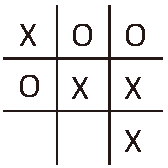
\includegraphics[width=4cm]{c1/img/tic-tac-toc.pdf}
\end{wrapfigure}
回想一下我们所熟悉的儿童游戏——井字棋<tic-tac-toc>. 两个玩家轮流在$3\times 3$的棋盘上下棋. 两个玩家轮流下\textsf{X}与\textsf{O}, 直到一个玩家在水平方向上、垂直方向上或对角线方向上放置了一排的三枚棋子以赢得游戏, 如图中X所做的那样. 如果棋盘填满了而没有任何一名玩家放置出一排三枚棋子, 那么该局比赛就是平局. 因为一名有经验的玩家永远不会输, 让我们假设我们在和一名下棋技术不完美的玩家对战, 他有时会下错来让我们赢得比赛. 让我们暂时假设平局和输掉比赛一样糟糕. 我们该怎样构建一个能发现对手的缺陷并最大化获胜概率的下棋程序呢?

虽然这是一个简单的问题, 但不能使用原有的技术来便利地、令人满意地解决. 例如, 博弈论中的典型的``极小化极大''<minimax>方法在这里是不适用的, 因为其假设了对手下棋的方式. 例如, 一个极小化极大程序永远不会到达一个可能会将其引向失败的状态, 即使在多数情况下因为对手的失误该状态会将其引向胜利. 典型的针对一系列决策问题的优化方法, 例如动态规划<dynamic programming>, 可以\emph{计算}出针对任一对手的方案, 但需要关于对手的完整说明——包括在棋盘的每一个状态中对手下任意一步棋的概率——作为输入. 让我们假设如同实际关注中的多数问题, 这些信息并非先验的. 另一方面, 通过和同一个对手下多盘棋, 这样的信息可以从经验中被评估出来. 对经典方法而言, 关于此问题能做到的最好的就是先学习得到有一定置信度的对手行为模型,  然后对给定的对手近似模型应用动态规划来计算最优解. 最后的这种方法, 和我们之后在本书中探讨的一些强化学习方法没有太大差别.

如果在本问题上应用进化方法, 那么其将在直接在策略空间中搜索可以以高概率战胜对手的策略. 其中, 一个策略即为指导玩家在每一个游戏状态——每一个在$3 \times 3$的棋盘上合法的\textsf{X}与\textsf{O}的配置——中该怎么走的规则. 对于每一个所考虑的策略, 其获胜概率的估计值可以通过与对手下多盘棋来获得. 这样的估计将用于指导哪些策略能够之后继续被考虑. 一个典型的进化算法能在策略空间中逐步提升<hill-climb>, 不停产生并估计策略以获得增量式的改进. 此外, 维持并估计多个策略的遗传算法也可以被使用. 事实上数以百计的优化算法都可以被使用.

接来下讨论井字棋问题怎么利用值函数来处理. 首先我们为每一个可能的状态建立一张数值表. 表中每一个数值都是从该状态起获胜的概率的最新估计值. 我们将此作为每一个状态的\emph{值}<value>, 同时整张表就是学得的值函数. 如果当前, 从状态\textsf{A}起获胜概率的估计值比状态\textsf{B}高, 那么状态\textsf{A}的值比状态\textsf{B}高, 或者说状态\textsf{A}比状态\textsf{B}更``好''. 假设我们一直执\textsf{X}, 那么对所有有一排三枚\textsf{X}棋子的状态其获胜概率为1, 因为在这样的情况下我们已经赢了. 类似的, 对于所有有一排三枚\textsf{O}棋子的状态或平局, 其获胜概率为0, 因为我们已经不可能赢了. 我们将所有其他状态的初始值设为0.5, 表示我们猜测从这些状态起有50\%的概率获胜.

然后我们同对手玩许多盘棋. 为了选择下一步棋, 我们检查下了一步棋之后所有可能的状态(将当前棋盘上任一空填上后各对应一个状态), 然后在表中查找各个状态当前的估计值. 在多数情况下我们\emph{贪心}<greedy>地选择下一步棋, 选择能导向拥有最高值的状态的那步棋, 即选择胜率估计值最高那步棋. 然而, 我们偶尔随机地选择下一步棋. 这些棋被称为\emph{探索}<exploratory>步, 因为这让我们探索原先根本无法经历的状态. 游戏中一系列所考虑与所做出的下法, 被绘制在了\figref{1.1}中.

\begin{figure}[ht]
\begin{center}
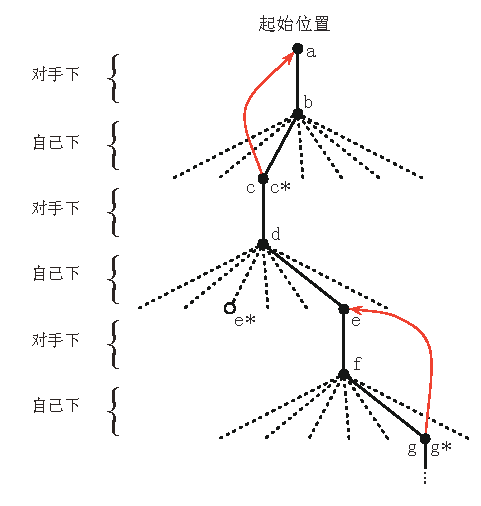
\includegraphics[width=0.7\textwidth]{c1/img/figure1-1.pdf}
\end{center}
\caption{一系列的井字棋下法. 实线表示游戏中实际所下; 虚线表示我们(我们的强化学习程序)考虑了, 但没有实际采用的下法. 我们下的第二步棋是一个探索步, 这意味着另一个同胞节点, 即那个$\mathrm e^*$对应的结点, 估计值更高. 探索步并不能造成学习; 但所有其他的步数可以, 这形成了如图中红色箭头所示的更新, 其中估计值从树的子孙结点流向祖先结点, 细节在正文中叙述.}\label{fig:1.1}
\end{figure}

当我们在下棋时, 我们更改我们经历过的状态的值. 我们尝试做出对获胜率更为准确的估计. 为了做到这一点, 我们将做出贪心选择后的状态值\emph{逆流}<back up>至做出贪心选择前的状态, 如\figref{1.1}所示. 更确切地说, 早先状态的当前值更新后向后续状态的值靠拢. 这可以通过将早先状态的值向后续状态接近部分做到. 让我们用$S_t$表示做出贪心选择前的状态, 用$S_{t + 1}$表示贪心选择后的状态, 那么对$S_t$的值的估计——记作$V(S_t)$——的更新可以写作:
\begin{equation*}
V(S_t) \leftarrow V(S_t) + \alpha[V(S_{t + 1}) - V(S_t)]​,
\end{equation*}
其中$\alpha$为称为\emph{步长}<step-size>的参数, 为一个小的正数, 能影响学习的速率. 上述的更新是\emph{时序差分}<temporal difference, TD>学习方法的特例, 时序差分名称的由来为——更新是基于$V(S_{t + 1}) - V(S_t)$这一两个连续状态的估计值之差.

上述的方法在这个问题上表现很好. 例如, 如果步长参数能随时间以合适的速率递减, 那么对于任何给定的对手, 任意状态的估计值都能收敛到从该状态起我方使用最优策略的话最终获胜的概率. 更进一步说, 收敛后所下的每一步(除去探索步)事实上都是针对这一(非完美)对手的最优下法. 换句话说, 此方法最终收敛为针对这一对手的最优策略. 如果步长参数没有随时间减小到0, 那么下棋程序也能很好地应对缓慢地改变策略的玩家.

这一例子阐明了进化方法与使用值函数的方法的区别. 为了评估一个策略, 进化方法使该策略固定, 同对手下许多盘棋或使用对手的模型模拟下许多盘棋. 获胜的频率给出了该策略获胜概率的无偏估计, 该频率可以用于指导下一步的策略选择. 但策略改进必须要经过许多盘游戏, 并且只有每局游戏的最终结果被利用了——发生在游戏\emph{过程中}的一切都被忽视了. 例如, 如果程序获胜了, 那么这局游戏中的\emph{所有}行为都获得了赞誉<credit>, 无论某一步对获胜而言有多重要. 赞誉甚至被给予从未下过的那几步. 而使用值函数的方法, 与之相反, 允许对各个状态分开进行评估. 从结果上而言, 进化方法与值函数方法都搜索了策略空间, 但对值函数的学习利用了游戏过程中的信息.

这个简单的例子阐明了强化学习方法的一些关键特征. 首先, 在有对手的情况下, 必须强调从与环境的交互中学习. 其次, 必须要有明确的目标, 且正确的动作选择需要将延迟的效果考虑在内的计划或远见. 例如, 简单的强化学习程序可能会学会由多步组成的陷阱, 来应对短视的对手. 这是强化学习方法的一个显著特征: 其不需要对手的模型, 也不需要对未来可能的动作、状态序列进行显式搜索, 就可以达到计划与预见的目的.

虽然这个示例阐明了一些强化学习的基本特征, 但它是在是太简单了, 以致于可能会给人留下强化学习的应用十分有限的印象. 除了井字棋这样的双人游戏外, 强化学习也可以用于没有形式上的对手的情形, 即``与自然斗争的游戏''. 虽然井字棋游戏中每一局是分开的且只在每一局的末尾有奖赏, 但强化学习并不局限于将交互划分为不同分节<episode>的问题. 强化学习也可以应用于交互是无穷无尽的情形, 或可以在任意时间接受不同量级的奖赏的情形. 强化学习甚至可以应用于不像井字棋那样将时间分为离散的步长的问题. 强化学习的一般准则也适用于连续时间<continuous-time>问题, 但相关理论同时也变得更复杂, 因此在此导论性质的书中略去.

虽然井字棋问题的状态集有限且元素数目较小, 但即使状态集很大乃至无限, 强化学习方法也依然适用. 例如, \citet{Tesauro1992, Tesauro1995}将上述算法同人工神经网络结合起来, 并用于有大约${10}^{20}$个状态的西洋双陆棋<backgammon>游戏. 对于这么多状态而言, 即使只经历其中的一小部分也是不可能的. Tesauro的程序的表现远比之前的任何程序好, 并最终超过了顶级人类玩家(\secref{16.1}). 人工神经网络为程序提供了对过去经验进行泛化的能力, 所以当面临新状态时, 程序能通过人工神经网络, 来根据过去面临的类似状态选择合适的下法. 在面临拥有如此庞大的状态集的问题时, 强化学习系统的性能同其能在多大程度上对过去的经验进行泛化密切相关. 在这个主题上, 强化学习最需要监督学习的方法. 为了做到这一点, 人工神经网络与深度学习(\secref{9.6})既不是唯一的方法, 也不一定是最好的方法.

井字棋游戏中, 在学习开始时没有除游戏规则外的任何先验知识, 但强化学习并不一定要从空白开始. 恰恰相反, 先验知识可以以多种方式集成到强化学习中, 且有时这对高效的学习而言是必需的(例如, 参见\secref{9.5}、\secref{17.4}及\secref{13.1}). 此外, 在井字棋游戏中我们可以获取到真实的状态信息, 但强化学习也可以应用于部分状态被隐藏的情形, 或者对学习器而言不同的状态看上去相同的情形.

最后, 井字棋程序能够预见未来, 并预测其所有可能的下法所引出的状态. 但是为了做到这一点, 强化学习程序需要游戏的一个模型, 该模型能预测环境对程序尚未走的那一步的可能反应. 许多问题都类似这样, 但在有些问题中甚至关于短期的动作效果的模型也无法得到. 强化学习在两种情况下都可以适用. 模型并不是必须的, 但如果有现成的模型或模型可以学得, 那么这些模型可以轻而易举地被使用(\chapref{8}).

在另一方面, 存在着不需要任何环境模型的强化学习方法. 免模型系统甚至无法预测环境对单个动作的反应. 使用TD方法的井字棋程序从对手的意义上说是免模型的: 其没有任何种类的关于对手的模型. 因为模型必须要足够准确才能派得上用场, 所以当解决问题的瓶颈在于难以构建足够准确的环境模型时, 免模型方法比其他更复杂的方法有优势. 免模型方法也是有模型方法的重要组件. 本书中, 我们先用数章讨论免模型方法, 然后再讨论其怎样作为更为复杂的有模型方法的组件.

强化学习方法既可以用于系统中的高层, 也可以用于系统中的底层. 虽然在井字棋程序仅学会了游戏的下法, 但没有什么能阻碍将强化学习用于更高的层次中, 其中可能每一个``动作''本身就是复杂的应用. 在层次化学习系统中, 强化学习可以同时工作于多个层级.

\begin{exer}[左右互搏]
假设如果强化学习算法并非与随机的对手对战, 而是自身左右互搏并且两边都进行学习. 你认为这种情况下会发生什么? 其能够学得不同的策略吗?
\end{exer}

\begin{exer}[对称性]
许多井字棋的走法看上去不一样, 但因为对称性的关系本质上是相同的. 我们该怎样修改上述的学习过程来利用这一点? 这一改变会以怎样的形式改善学习过程? 现在, 再思考另一个问题. 假设对手没有利用对称性. 那么在这种情况下, 我们应该利用对称性吗? 对称的位置一定有相等的值吗?
\end{exer}

\begin{exer}[贪心的下法]
假设强化学习程序是贪心的, 即其永远选择能带来最高值的下法. 那么其学得的策略会比非贪心程序更好还是更差? 什么样的问题可能会出现?
\end{exer}

\begin{exer}[从探索中学习]
假设在所有游戏中的所有步之后都进行更新, 包括探索步. 如果步长参数随时间流逝逐渐适当地减小(但探索的可能性不会), 那么各个状态的值会收敛至一个不同的胜率的集合. 从概念上说, 当从或者不从探索步中学习时, 这两个胜率的集合各自是什么? 假设我们继续做出探索步, 那么哪一个胜率的集合可能会更好? 哪一个可能会赢得更多?
\end{exer}

\begin{exer}[其他改进]
你可以想到其他改善强化学习程序的方式吗? 你可以想到更好的用于解决上述的井字棋问题的方法吗?
\end{exer}

\section{总结}\label{sec:1.6}

强化学习是理解并自动化目标导向的学习与决策的计算性方法. 与别的计算性方法的不同之处在于: 其强调从代理与环境的直接交互中学习, 而不需要示范性的训练集或环境的完整模型. 我们认为, 强化学习是第一个真正处理``从与环境的交互中学习来达成长期的目标''这一问题的学科. 

强化学习使用马尔科夫决策过程这一框架, 依据状态、动作与奖赏来定义学习代理与环境之间的交互. 这一框架试图以一种简单的方式表示人工智能问题中的关键特征. 这些特征包括对因果的理解, 对不确定性与概率性的理解, 以及存在有明确的目标.

值与值函数的概念是本书中介绍的多数强化学习方法的关键. 我们认为值函数对于在策略空间中的高效搜索而言是至关重要的. 值函数的使用将强化学习方法同进化方法区别开来, 其中后者通过对整个策略的评估来在策略空间中进行直接搜索.

\section{强化学习的早期历史}\label{sec:1.7}

暂不译

\section*{参考文献}

暂无

